\documentclass{article}

\usepackage{amsmath}
\usepackage{amssymb}
\usepackage{graphicx}
\usepackage{tikz}
\usetikzlibrary{arrows}
\usepackage{verbatim}
%\usepackage{sfmath}
\usepackage{psfrag}
\usepackage{here} 
\usepackage{hyperref}
\usepackage{xcolor}
\usepackage{tcolorbox}
\usepackage{physics}


%\textheight=24cm

%\renewcommand\sfdefault{phv}     %use helvetica for sans serif
\renewcommand{\familydefault}{\sfdefault}
\renewcommand{\familydefault}{cmss}

\title{Práctica 1}
\author{Javier Izquierdo Hernández}
\date{\today}
\begin{document}
	\begin{titlepage}
		\centering
		{
\includegraphics[width=0.3\textwidth]{figures/logo}\par}
		\vspace{1cm}
		{\bfseries\LARGE Universidad Rey Juan Carlos \par}
		\vspace{1cm}
		{\scshape\Large E.T.S. Ingeniería de Telecomunicación \par}
		\vspace{3cm}
		{\scshape\Huge Ingeniería de Control \par}
		\vspace{3cm}
		{\itshape\Large Práctica 1 \par}
		\vfill
		{\Large Autor: \par}
		{\Large Javier Izquierdo Hernández \par}
		\vfill
		{\Large \today \par}
	\end{titlepage}
\begin{center}
{\huge \bf Práctica 1}
\end{center}


Consider the system represented in Figure~\ref{fig:figure_1}, composed of a sphere $S$ of radius $r$ and barycentric moment of inertia $J_S$ placed on a rod $B$ of length $l$ and barycentric moment of inertia $J_B$, which is hinged exactly at the center of mass $O$. 
$p$ indicates the position in m of the contact point between the sphere and the rod with respect to the hinge point. It is zero at the hinge point $O$ and positive to the right.
$\theta$ and $\theta_S$ indicate the angular position in rad of the rod and the sphere, respectively. 
$\dot{\theta}$ and $\dot{\theta}_S$ indicate the angular velocity in rad/s of the rod and the sphere, respectively. $u$ is the control torque expressed in $\text{kg m}$.


\begin{figure}[H]
\centerline{\hspace{1.25cm}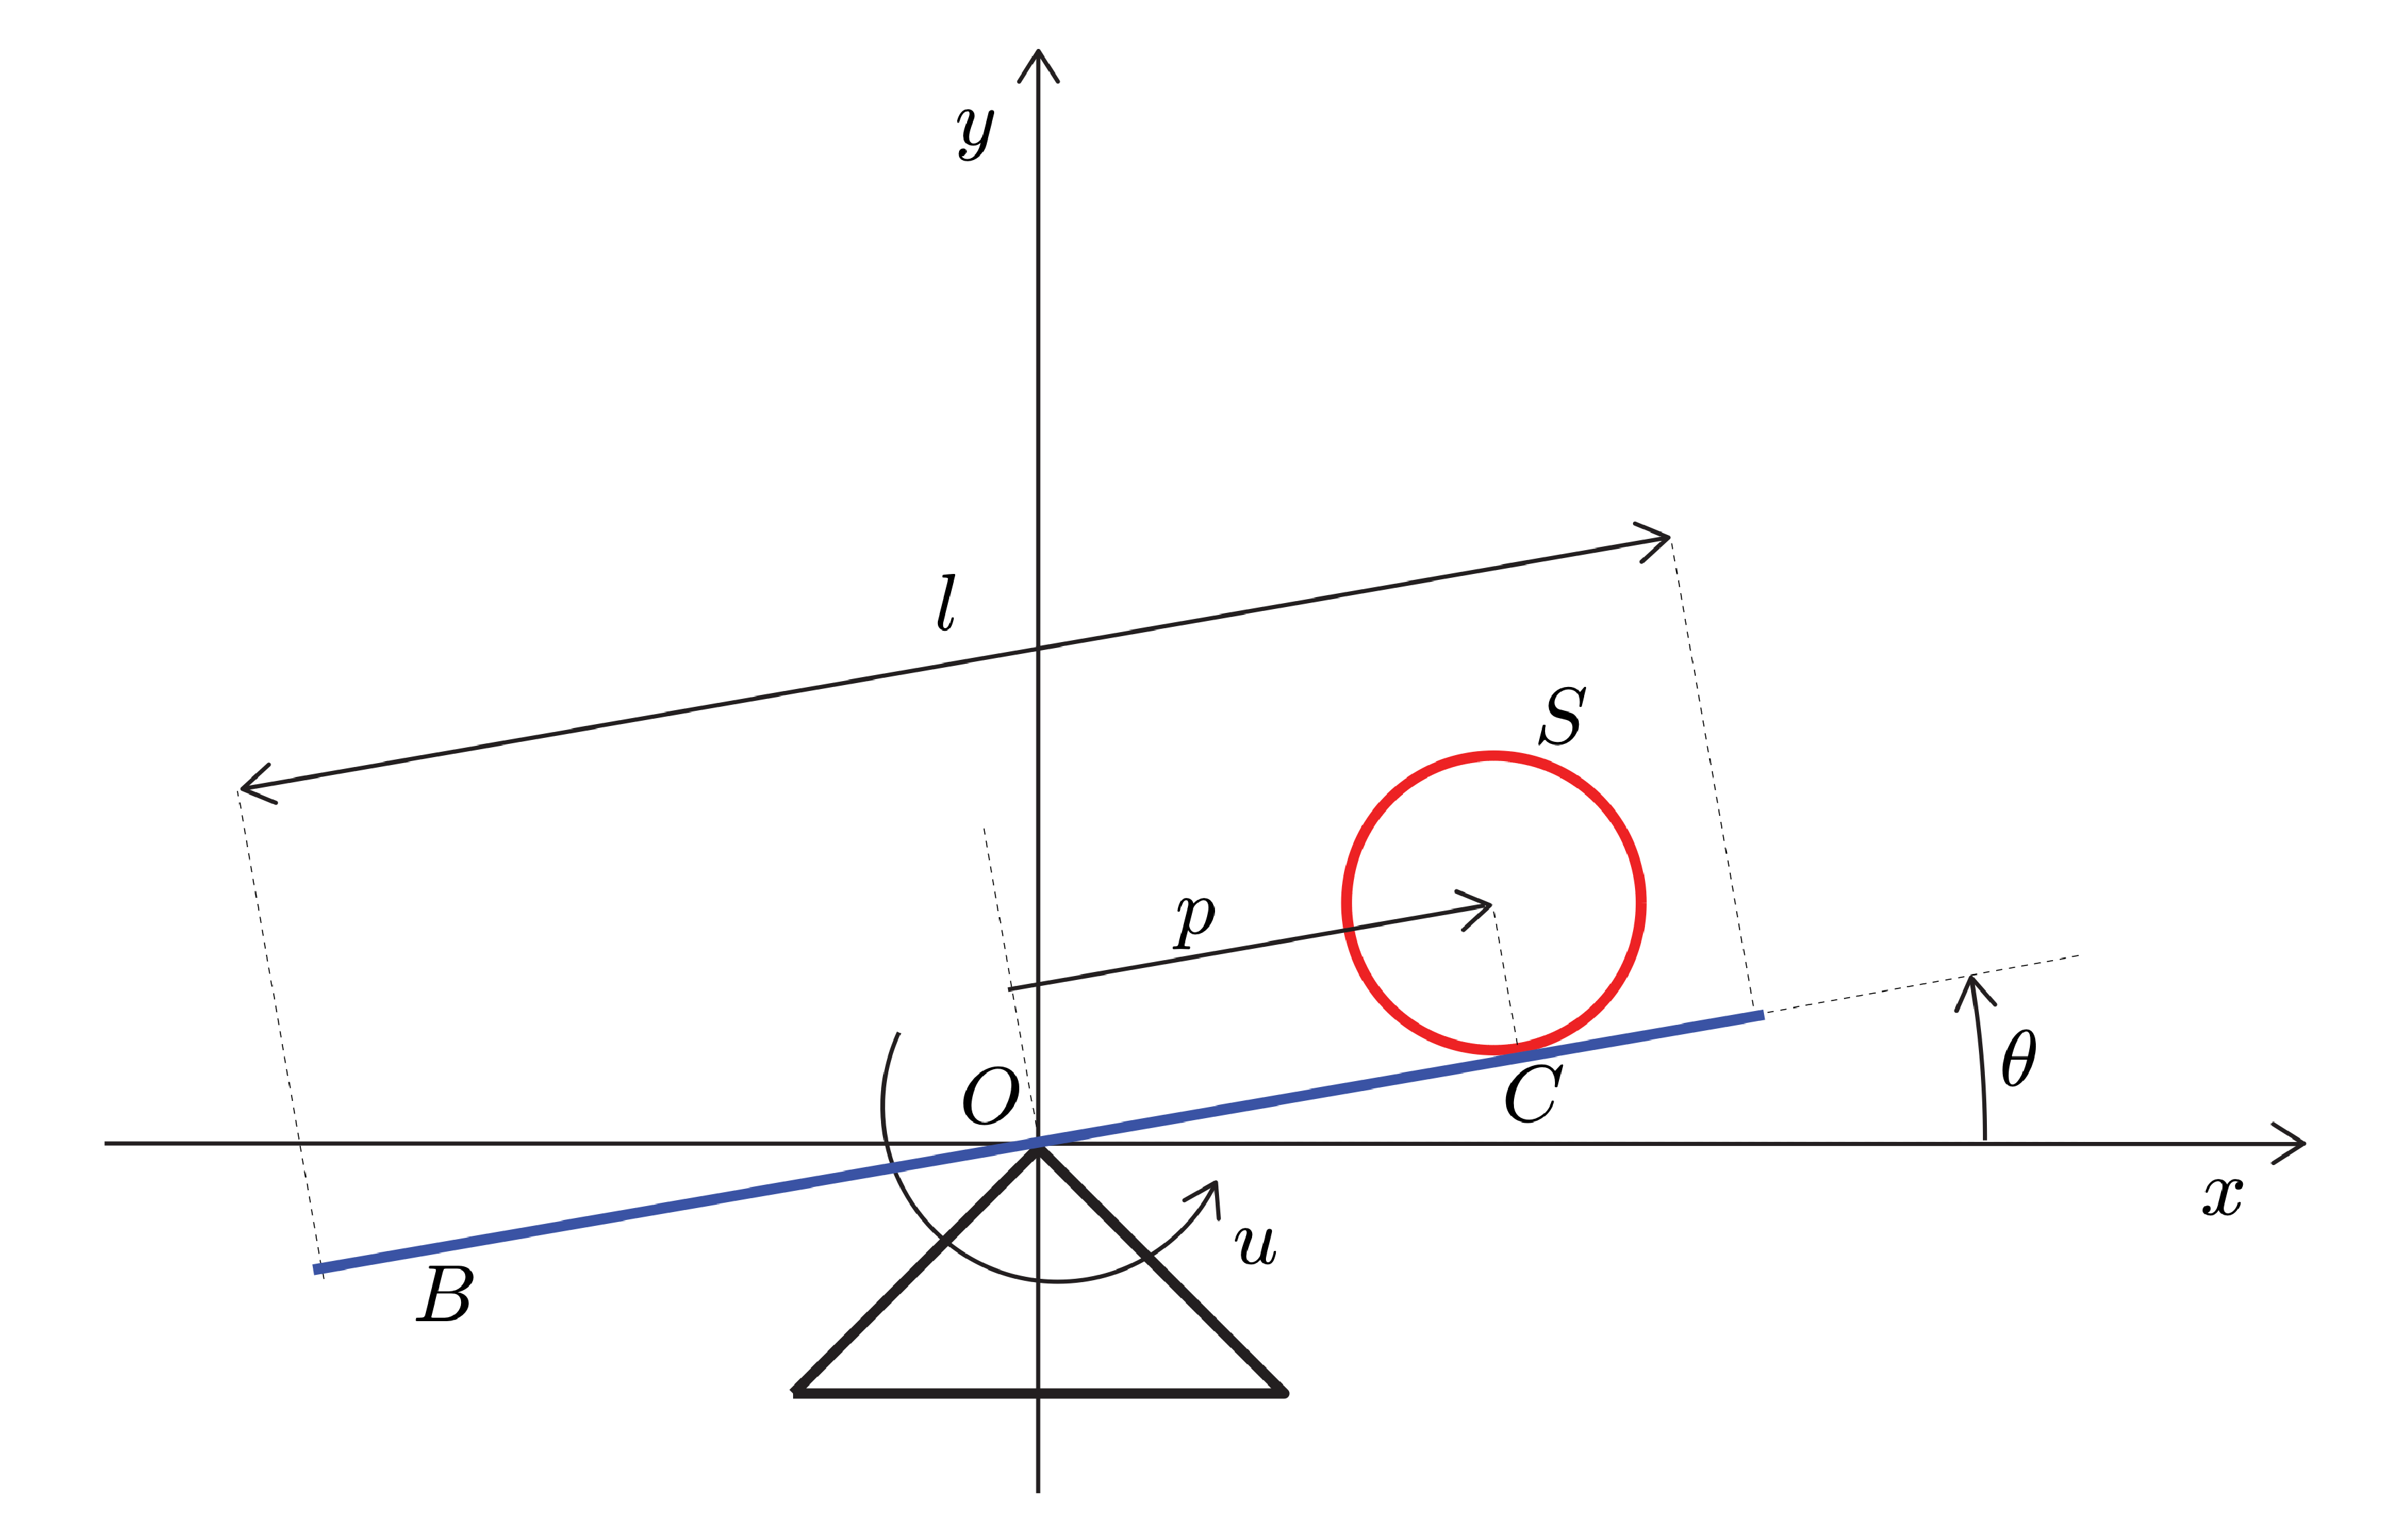
\includegraphics[width=0.8\columnwidth]{figures/figure_1_a}}
\caption{Sketch of the system.}
\label{fig:figure_1}
\end{figure}


\renewcommand{\thefigure}{2}



The dynamic model of this system is
\begin{eqnarray*}
(J_B + m_S \, p^2) \ddot{\theta}  + 2 \, m_S \, p \, \dot{p} \, \dot{\theta}  + m_S \, g \, p \cos \theta &=&u, \\
\left( m_S + \frac{J_S}{r^2} \right) \ddot{p}  - m_S \, p \, \dot{\theta}^2   + m_S g \sin \theta &=&0,
\end{eqnarray*}
with the following parameters 
\begin{itemize}
\item
length of the rod: $l=0.5 \; \text{m}$,
\item
barycentric moment of inertia of the rod: $J_B = 2.4 \; \text{kg m}^2$, 
\item
radius of the sphere: $r = 0.05 \; \text{m}$,
\item
mass of the sphere: $m_S = 1.25 \; \text{kg}$, 
\item
barycentric moment of inertia of the sphere: $J_S = 40 \cdot 10^{-3} \; \text{kg m}^2$,
\item
gravity acceleration: $g = 9.81 \; \text{m}/\text{s}^2$.
\end{itemize}



















\begin{itemize}
\item[1)] Demonstrate the equations of the dynamic model using the Lagrange method.
(Contesta en el informe)

\item[2)] Calculate the state space representation of the system, assuming that $\mathbf{x} = (\theta, p, \dot{\theta}, \dot{p})^T = ( x_1,x_2,x_3,x_4)^T$ and that only the position $x_2$ of the sphere is measured.
(Contesta en el informe y sube el c\'odigo \texttt{Matlab} a Aula Virtual en el fichero answer\_2.m)



\end{itemize}

\bigskip

\noindent
{\color{red} Write a detailed report answering each question in a different section. 

\bigskip


\noindent
Originality and completeness of the answers will be the aspects that will be taken into account in the grading of the report, and therefore, the \texttt{Matlab} code alone will not be considered.} 

\newpage
\section*{Informe}
\begin{itemize}
	\item[1)] Demonstrate the equations of the dynamic model using the Lagrange method.
	
	Para poder demostrar las ecuaciones del modelo dinámico con el método de Lagrange necesitamos hallar la diferencia entre la energía cinética del sistema \textit{T} y la energía potencial \textit{V} para conseguir $L = T - V$.\\
	Las ecuaciones de Lagrange son:
	\begin{center}
		$\frac{d}{dt}\pdv{L}{\dot{x_{i}}}-\pdv{L}{x_{i}}=f_{i},$\hspace{20pt}$i = 1, 2, ..., n$	
	\end{center}
	donde $x_{i}$ representa a la i-nésima variables y $f_{i}$ es la i-nésima fuerza aplicada al sistema.\\
	En este caso las 2 variables son:
	\begin{itemize}
		\item $\theta$ el ángulo de inclinación de la barra.
		\item \textit{p} la distancia desde el centro de la esfera al centro de la barra.
	\end{itemize}
	Y también tendriamos sus derivadas $\dot{x}$:
	\begin{itemize}
		\item $\dot{\theta}$ la velocidad angular de la barra.
		\item $\dot{p}$ la velocidad de la esfera.
	\end{itemize}
	Ahora calculamos la energía cinética $T$:
	\begin{itemize}
		\item Barra, solo tiene de rotación porque solo rota sobre si misma: 
		\begin{center}
			$T_{B} = \frac{1}{2}J_{B}\dot{\theta}^2$
		\end{center}
		\item Esfera, componente de rotación porque la esfera rota:
		\begin{center}
			$T_{S_{Rot}} = \frac{1}{2}J_{S}\dot{\theta_{S}}^2$
		\end{center}
		\item Esfera, componente lineal en x porque se mueve sobre el eje x: 
		\begin{center}
			$T_{S_{Lin_{x}}} = \frac{1}{2}m_{s}(\frac{d}{dt}(p\ cos(\theta)))^2$	
		\end{center}
		\item Esfera, componente lineal en y porque se desplaza en el eje y: 
		\begin{center}
			$T_{S_{Lin_{y}}} = \frac{1}{2}m_{s}(\frac{d}{dt}(p\ sin(\theta)))^2$
		\end{center}
		\item Esfera:
		\begin{center} 
			$T_{S} = T_{S_{Rot}} + T_{S_{Lin_{x}}} + T_{S_{Lin_{y}}}$
		\end{center}
	\end{itemize}
	Como se puede apreciar, la componente lineal de la esfera ha sido dividida en 2 ya que se mueve sobre los 2 ejes, no solo en uno.\\
	\begin{center}
		$T = T_{B} + T_{S} = \frac{1}{2}J_{B}\dot{\theta}^2 + \frac{1}{2}J_{S}\dot{\theta_{S}}^2 + \frac{1}{2}m_{s}(\frac{d}{dt}(p\ cos(\theta)))^2 + \frac{1}{2}m_{s}(\frac{d}{dt}(p\ sin(\theta)))^2 = 
		 \frac{1}{2}J_{B}\dot{\theta}^2 + \frac{1}{2}J_{S}\dot{\theta_{S}}^2 + \frac{1}{2}m_{s}(\dot{p}\ cos(\theta) - p\dot{\theta}sin(\theta))^2 + \frac{1}{2}m_{s}(\dot{p}\ sin(\theta) + p\dot{\theta}cos(\theta))^2 = 
		 \frac{1}{2}J_{B}\dot{\theta}^2 + \frac{1}{2}J_{S}\dot{\theta_{S}}^2 + \frac{1}{2}m_{S}\dot{p}^2 + \frac{1}{2}m_{S}p^2\dot{\theta}^2
		 $
	\end{center}
	Como $\dot{\theta_{S}} = \frac{\dot{p}}{r}$, sustituimos para tener todo en función de $\theta$ y $p$:
		\begin{center}
		$T = 
		\frac{1}{2}J_{B}\dot{\theta}^2 + \frac{1}{2}\frac{J_{S}}{r^2}\dot{p}^2 + \frac{1}{2}m_{S}\dot{p}^2 + \frac{1}{2}m_{S}p^2\dot{\theta}^2
		$
	\end{center}
	Luego obtenemos la energía potencial del sistema $V$. Solo la esfera tiene energía potencial:
	\begin{center}
		$V = m_{S}\ g\ p\ sin(\theta)$
	\end{center}
	Con esto obtenemos que la \textit{Lagrangean} es:
	\begin{center}
		$L = T - V
		 = \frac{1}{2}J_{B}\dot{\theta}^2 + \frac{1}{2}\frac{J_{S}}{r^2}\dot{p}^2 + \frac{1}{2}m_{S}\dot{p}^2 + \frac{1}{2}m_{S}p^2\dot{\theta}^2 - m_{S}\ g\ p\ sin(\theta)
		$
	\end{center}
	Luego las ecuaciones de Lagrange son (La primera es 0 porque el sistema está en equilibrio):
	\begin{center}
		$\frac{d}{dt}\pdv{L}{\dot{p}}-\pdv{L}{p}=0$\\
		$\frac{d}{dt}\pdv{L}{\dot{\theta}}-\pdv{L}{\theta}=u$
	\end{center}
	De
	\begin{center}
		$\frac{d}{dt}\pdv{L}{\dot{p}}-\pdv{L}{p}=0$,
	\end{center}
	tenemos
	\begin{center}
		$\pdv{L}{\dot{p}}= m_{S}\dot{p} + \frac{J_{S}}{r^2}\dot{p}$,\\
		$\frac{d}{dt}\pdv{L}{\dot{p}}= (m_{S} + \frac{J_{S}}{r^2})\ddot{p}$,\\
		$\pdv{L}{p}= m_{S}p\dot{\theta}^2 - m_{S}\ g\ sin(\theta)$
	\end{center}
	La primera ecuación de Lagrange es
	\begin{center}
		$\frac{d}{dt}\pdv{L}{\dot{p}}-\pdv{L}{p}= (m_{S} + \frac{J_{S}}{r^2})\ddot{p} - m_{S}p\dot{\theta}^2 + m_{S}\ g\ sin(\theta) = 0$
	\end{center}
	
	Igualmente de
	\begin{center}
		$\frac{d}{dt}\pdv{L}{\dot{\theta}}-\pdv{L}{\theta}=u$,
	\end{center}
	tenemos
	\begin{center}
		$\pdv{L}{\dot{\theta}}= m_{S}\dot{\theta}p^2 + J_{B}\dot{\theta}$,\\
		$\frac{d}{dt}\pdv{L}{\dot{\theta}}= (m_{S}p^2 + J_{B})\ddot{\theta} + 2m_{S}p\ \dot{p}\ \dot{\theta}$,\\
		$\pdv{L}{\theta}=- m_{S}\ g\ p\ cos(\theta)$
	\end{center}
	La segunda ecuación de Lagrange es
	\begin{center}
		$\frac{d}{dt}\pdv{L}{\dot{\theta}}-\pdv{L}{\theta}=(m_{S}p^2 + J_{B})\ddot{\theta} + 2m_{S}p\ \dot{p}\ \dot{\theta} + m_{S}\ g\ p\ cos(\theta)=u$
	\end{center}
	Luego tenemos que las ecuaciones de Lagrange son:
	\begin{center}
		$\frac{d}{dt}\pdv{L}{\dot{p}}-\pdv{L}{p}= (m_{S} + \frac{J_{S}}{r^2})\ddot{p} - m_{S}p\dot{\theta}^2 + m_{S}\ g\ sin(\theta) = 0$\\
		$\frac{d}{dt}\pdv{L}{\dot{\theta}}-\pdv{L}{\theta}=(m_{S}p^2 + J_{B})\ddot{\theta} + 2m_{S}p\ \dot{p}\ \dot{\theta} + m_{S}\ g\ p\ cos(\theta)=u$
	\end{center}
	Como son iguales que las del modelo dinámico podemos decir que las hemos demostrado de manera correcta.
	\item[2)] Calculate the state space representation of the system, assuming that $\mathbf{x} = (\theta, p, \dot{\theta}, \dot{p})^T = ( x_1,x_2,x_3,x_4)^T$ and that only the position $x_2$ of the sphere is measured.\\
	Para calcular la representación del estado de espacios introducimos 4 variables $x_{1}(t)$, $x_{2}(t)$, $x_{3}(t)$, $x_{4}(t)$ y definimos que $x_{1}(t) = \theta(t)$, $x_{2}(t)=p$, $x_{3}(t) = \dot{\theta(t)}$, $x_{4}(t)=\dot{p}$. Por lo tanto,
	\begin{center}
		$x(t) = \begin{pmatrix}
			x_{1}(t)   \\       
			x_{2}(t)     \\     
			x_{3}(t)\\   
			x_{4}(t)\\   
		\end{pmatrix} = 
		\begin{pmatrix}
		\theta    \\       
		p      \\     
		\dot{\theta} \\   
		\dot{p}\\ 
		\end{pmatrix}$
	\end{center}
	Y como tenemos la segunda derivada lo podemos expresar como
	\begin{center}
		$\frac{d}{dt}\begin{pmatrix}
			\theta(t)    \\       
			p(t)      \\     
			\dot{\theta}(t) \\   
			\dot{p}(t)\\ 
		\end{pmatrix} = \begin{pmatrix}
			\dot{\theta}(t)   \\       
			\dot{p}(t)      \\     
			\ddot{\theta}(t) \\   
			\ddot{p}(t)\\ 
		\end{pmatrix} = 
		\begin{pmatrix}
			\dot{\theta}(t)   \\       
			\dot{p}(t)      \\     
			\frac{-2m_{S}\ p(t)\ \dot{p}(t)\ \dot{\theta}(t) - g\ m_{S}\ p(t)\ cos(\theta(t))+ u(t)}{J_{B} + m_{S}\ p(t)} \\   
			\frac{m_{S}\ p(t)\ \dot{\theta}^2(t) + g\ m_{S}\ sin(\theta(t))}{\frac{J_{S}}{r^2} + m_{S}}\\ 
		\end{pmatrix}$
	\end{center}
	Luego la representación del espacio de estados es
	\begin{center}
		$\dot{x_{1}} = x_{3}(t)$\\
		$\dot{x_{2}} = x_{4}(t)$\\
		$\dot{x_{3}} = \frac{-2m_{S}\ x_{2}(t)\ x_{4}(t)\ x_{3}(t) - g\ m_{S}\ p\ cos(x_{1}(t))+ u(t)}{J_{B} + m_{S}\ x_{2}(t)}$\\
		$\dot{x_{4}} = \frac{m_{S}\ x_{2}(t)\ x_{3}^2 + g\ m_{S}\ sin(x_{1}(t))}{\frac{J_{S}}{r^2} + m_{S}}$\\
	\end{center}	

\end{itemize}
\newpage
\section*{Solution}




\noindent
    \begin{tcolorbox}[
        title={File \texttt{answer\_2.m}},
%        halign=center,
%        valign=center,
%        nobeforeafter,
        width=13cm,
    ]
    
\begin{scriptsize}
\begin{verbatim}

close all
clc

syms theta thetadot thetaddot p pdot pddot ms Jb Js r g u;

% Known variables
%Jb = 2.4;
%Js = 0.040;
%ms = 1.25;
%g = 9.81;
%r = 0.05;

% State space representation x = [theta, p, thetadot, pdot];

% Define the dynamic equations
ecuaciones = [(ms*p + Jb)*thetaddot+2*ms*p*pdot*thetadot+ms*g*p*cos(theta)-u==0,
(ms+Js/r^2)*pddot-ms*p*thetadot^2+ms*g*sin(theta)==0];

% Solve thetaddot and pddot
[thetaddot, pddot] = solve (ecuaciones,[thetaddot, pddot]);

% Do the derivative to thetaddot and pddot
pdot = diff(pddot);
thetadot = diff(thetaddot);

% State representation
xdot = [thetadot, pdot, thetaddot, pddot]

\end{verbatim}
\end{scriptsize}
\end{tcolorbox}




\end{document}
